\documentclass[11pt,a4paper]{article}
\usepackage[margin=1in]{geometry}
\usepackage{amsmath,amssymb}
\usepackage{booktabs}
\usepackage{graphicx}
\usepackage{float}
\usepackage[hidelinks]{hyperref}
\usepackage{titlesec}
\usepackage{placeins}
\usepackage{caption}
\captionsetup{font=small,labelfont=bf}
\setlength{\parskip}{0.4em}
\setlength{\parindent}{0pt}
\setlength{\textfloatsep}{8pt plus 2pt minus 2pt}
\setlength{\intextsep}{8pt plus 2pt minus 2pt}
\setlength{\abovecaptionskip}{4pt}
\setlength{\belowcaptionskip}{2pt}
\titleformat{\section}{\large\bfseries}{\thesection}{1em}{}
\titleformat{\subsection}{\normalsize\bfseries}{\thesubsection}{1em}{}

\title{\vspace{-3em}\textbf{Order Flow Imbalance and Price Impact in CME Ether Futures}}
\author{Tony Li\thanks{Independent research conducted by the author; the views expressed are the author's own and not those of Imperial College London.}\\ \normalsize Imperial College London}
\date{August 2026}

\begin{document}
\maketitle

\begin{abstract}
\noindent We study Order Flow Imbalance (Cont, Kukanov, and Stoikov, 2014) on CME Ether futures over February 2021 to August 2026. On 28{,}711 out-of-sample dollar-volume bars, an OLS regression of bar mid-quote change on contemporaneous OFI with Newey-West HAC standard errors yields $\hat{\beta}_0 = +0.215$ ($t = 58.1$, $R^2 = 0.30$), against $+0.300$ and $R^2 = 0.31$ in sample. The regression is contemporaneous, so it measures price impact rather than forecasting power: used on its own as a predictor, lagged OFI explains essentially none of the following bar's move ($R^2 < 0.001$ out of sample). OFI is a strong descriptor of price formation on this contract; it is not, by itself, a trading signal.
\end{abstract}

\section{Introduction}

Order Flow Imbalance (OFI) aggregates best-bid and best-offer quote arrivals into a signed measure of top-of-book pressure. On liquid US equities, contemporaneous OFI explains roughly two-thirds of bar-level mid-quote variation (Cont, Kukanov, and Stoikov, 2014). The cryptocurrency evidence is thinner: Silantyev (2019) finds trade-flow imbalance dominates short-horizon prices on BitMEX XBT/USD, and Bieganowski and Ślepaczuk (2026) report OFI as the top SHAP feature in CatBoost ensembles on Binance Futures perpetuals. CME's Ether contract sits apart from both: a regulated venue whose quoted spread, in basis points of price, is an order of magnitude wider than the equity tape's.

This paper estimates the contemporaneous OFI--price relation on CME ETH futures from February 2021 to August 2026. The construction is the level-1 (best bid / best offer) form of Cont, Kukanov, and Stoikov on dollar-volume bars built from TBBO (trade-sampled top-of-book) events (Lopez de Prado, 2018).

\section{Data}

The panel consists of CME-cleared TBBO data for the front-month ETH futures contract, covering February 2021 through August 2026, with rolls handled by contract stitching.

Bars are constructed in dollar volume, with the threshold calibrated so that a median in-sample trading day produces about ten bars, and that threshold is held fixed when bars are constructed for the out-of-sample period.

For each bar the following quantities are computed:
\begin{itemize}
    \item \texttt{ofi}: signed level-1 (best bid / best offer) order flow imbalance, following the construction of Cont, Kukanov, and Stoikov (2014). For each TBBO update $i$, let $p^B_i, p^A_i$ denote the best-bid and best-ask quotes and $q^B_i, q^A_i$ their sizes. The per-event OFI contribution is $e_i = e^B_i + e^A_i$, where
    \begin{align*}
    e^B_i &=
    \begin{cases}
        +q^B_i              & \text{if } p^B_i > p^B_{i-1}  \\
        -q^B_{i-1}          & \text{if } p^B_i < p^B_{i-1}  \\
        q^B_i - q^B_{i-1}   & \text{if } p^B_i = p^B_{i-1}
    \end{cases},
    \qquad
    e^A_i =
    \begin{cases}
        -q^A_i              & \text{if } p^A_i < p^A_{i-1}  \\
        +q^A_{i-1}          & \text{if } p^A_i > p^A_{i-1}  \\
        -(q^A_i - q^A_{i-1})& \text{if } p^A_i = p^A_{i-1}.
    \end{cases}
    \end{align*}
     The bar OFI is the unnormalised sum over all events in the bar, $O_t = \sum_{i \in \text{bar } t} e_i$.
    \item \texttt{mid\_close}: the mid quote $(p^B + p^A)/2$ at the bar boundary.
    \item \texttt{d\_mid}: the change in mid quote since the previous bar.
\end{itemize}

\section{Signal-impact regression}
\label{sec:impact}

Following Cont, Kukanov, and Stoikov (2014) and Silantyev (2019), bar mid-quote change is regressed on contemporaneous and one-bar lagged OFI:
\begin{equation}
\Delta p_t = \alpha + \beta_0 \, O_t + \beta_1 \, O_{t-1} + \varepsilon_t,
\end{equation}
where $\Delta p_t = m_t - m_{t-1}$ is the change in mid-quote between bar boundaries and $O_t$ is the bar OFI, so $\beta_0$ is in dollars of mid-quote change per contract of net imbalance. Standard errors are Newey-West HAC (Newey and West, 1987) with five lags. Table~\ref{tab:impact} reports the estimates on the full panel, the 2021-02 to 2023-12 in-sample (IS) window, and the 2024-01 to 2026-08 out-of-sample (OOS) window.

\begin{table}[H]
\centering
\small
\begin{tabular}{lrrrrrr}
\toprule
Window & $n$ (bars) & $\hat\beta_0$ & HAC $t(\beta_0)$ & $\hat\beta_1$ & HAC $t(\beta_1)$ & $R^2$ \\
\midrule
Full sample            & 41{,}055 & $+0.247$ & $+70.2$ & $-0.027$ & $-14.4$ & 0.29 \\
In-sample 2021--23     & 12{,}344 & $+0.300$ & $+44.9$ & $-0.025$ & $-7.0$  & 0.31 \\
Out-of-sample 2024--26 & 28{,}711 & $+0.215$ & $+58.1$ & $-0.026$ & $-13.3$ & 0.30 \\
\bottomrule
\end{tabular}
\caption{OLS, Newey-West HAC (five lags). $p < 10^{-6}$ on both coefficients in every window.}
\label{tab:impact}
\end{table}

Both subsamples reject $\beta_0 = 0$ at $p < 10^{-6}$ (Figure~\ref{fig:impact}). The IS and OOS $R^2$ are nearly identical ($0.31$ and $0.30$), while the slope itself is less stable, moving from $+0.300$ in-sample to $+0.215$ out-of-sample. Both $R^2$ figures are below the two-thirds level of Cont et al.\ (2014) for liquid US equities.

\begin{figure}[t]
\centering
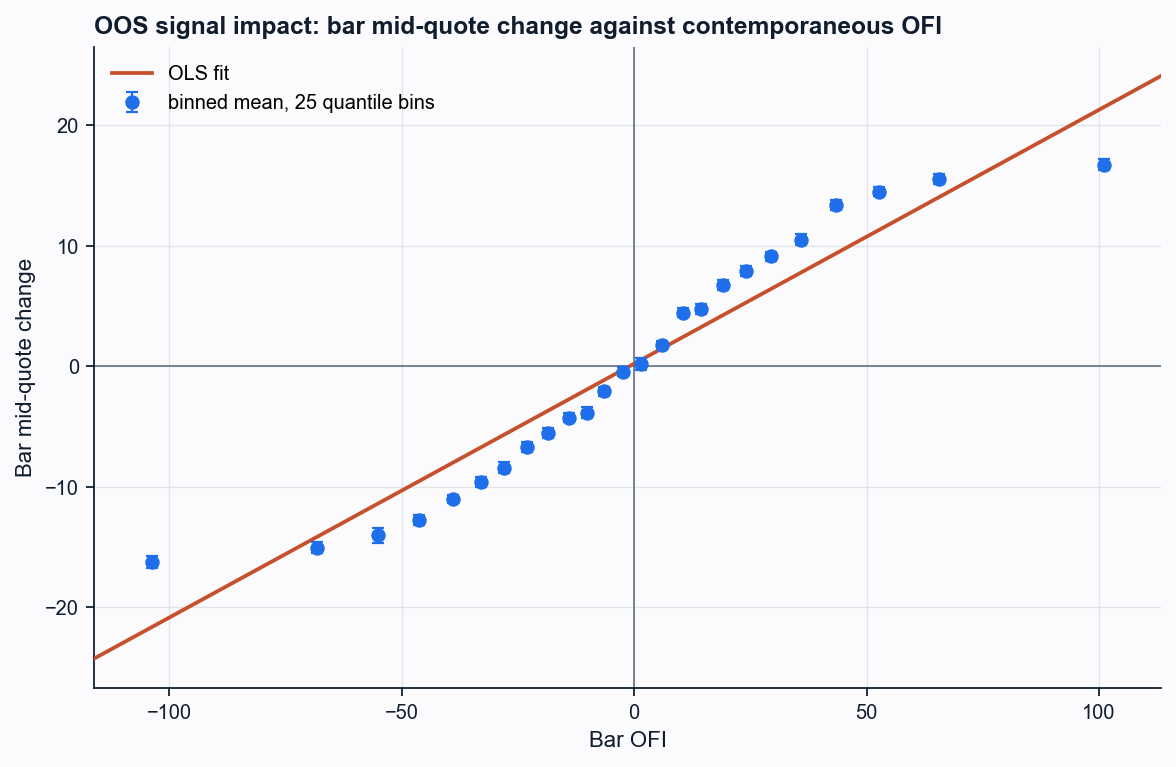
\includegraphics[width=0.88\textwidth]{fig5_impact.png}
\caption{Out-of-sample bar mid-quote change against contemporaneous OFI, 25 quantile bins with $\pm1$ standard error and the OLS fit. The relationship is monotonic, with impact per unit of flow attenuating at extreme flows --- both tail bins fall inside the straight-line fit; full estimates are in Table~\ref{tab:impact}.}
\label{fig:impact}
\end{figure}

This regression is contemporaneous: it measures how the mid quote moves together with the flow inside a bar (mean OOS bar duration ${\approx} 49$ minutes), not whether flow forecasts the next bar. Used on its own as a predictor, lagged OFI explains essentially none of the following bar's move ($R^2 < 0.001$ out-of-sample), so the content of Table~\ref{tab:impact} is price impact rather than forecastability. Whether the flow carries predictive content at horizons inside the bar is a question the bar regression cannot resolve, and answering it properly requires quote-level data.

\section{Conclusion}

The contemporaneous OFI--price relation is strong and stable on CME Ether futures: the explanatory power is nearly identical in and out of sample ($R^2$ of $0.31$ and $0.30$), and the slope remains large and precisely estimated throughout. It is a statement about price impact, not forecastability --- lagged OFI alone explains essentially none of the next bar's move --- so the result describes how this market absorbs order flow rather than offering a trading signal.

The tape bounds what can be measured. TBBO is trade-sampled, so the book is observed only when a trade prints, and it carries no depth beyond the touch. A quote-level feed would permit measuring the relation at horizons inside the bar --- where any predictive content would live --- and a proper treatment of execution, which are the natural extensions.

\section*{References}

\begin{itemize}
    \setlength{\itemsep}{0.2em}
    \item Bieganowski, B. and Ślepaczuk, R. (2026). Explainable patterns in cryptocurrency microstructure. arXiv:2602.00776.
    \item Cont, R., Kukanov, A., and Stoikov, S. (2014). The price impact of order book events. \textit{Journal of Financial Econometrics}, 12(1), 47--88.
    \item Lopez de Prado, M. (2018). \textit{Advances in Financial Machine Learning}. Wiley.
    \item Newey, W.~K. and West, K.~D. (1987). A simple, positive semi-definite, heteroskedasticity and autocorrelation consistent covariance matrix. \textit{Econometrica}, 55(3), 703--708.
    \item Silantyev, E. (2019). Order flow analysis of cryptocurrency markets. \textit{Digital Finance}, 1(1), 191--218.
\end{itemize}

\end{document}
